\documentclass[12pt, twoside]{article}
\usepackage[letterpaper, margin=1in, headsep=0.5in]{geometry}
\usepackage[english]{babel}
\usepackage[utf8]{inputenc}
\usepackage{amsmath}
\usepackage{amsfonts}
\usepackage{amssymb}
\usepackage{tikz}
\usetikzlibrary{quotes, angles}
\usepackage{graphicx}
%\usepackage{pgfplots}
%\pgfplotsset{width=10cm,compat=1.9}
%\usepgfplotslibrary{statistics}
%\usepackage{pgfplotstable}
%\usepackage{tkz-fct}
%\usepackage{venndiagram}
\usepackage{enumitem}
\usepackage{multicol}

\usepackage{fancyhdr}
\pagestyle{fancy}
\renewcommand{\headrulewidth}{0pt} % disable the underline of the header

\fancyhead[RO]{Name: \hspace{1.5in}}
\lhead{BECA / Dr. Huson / 10th Grade Geometry\\* Learning trajectory: Angle pairs}

\renewcommand{\headrulewidth}{0pt}

\begin{document}
\subsubsection*{Angle pairs and angle measure calculations}
  \begin{enumerate}
  \item Notation and terminology
  \item Complementary and supplementary calculations
  \item Algebraic solutions of pair situations
  \begin{enumerate}
    \item Linear pairs
    \item Vertical angles
    \end{enumerate}
  \item Triangle exterior angles
  \end{enumerate}

\subsubsection*{Draw a linear pair with given measure}
  \begin{enumerate}
    \item Given opposite rays $\overrightarrow{AB}$ and $\overrightarrow{AC}$, with $\overline{AB}=6$ cm. Draw a ray $\overrightarrow{AD}$ such that $m \angle BAD=60^\circ$ and $\overline{AD}=6$ cm.
    %\vspace{7cm}
    \begin{center}
    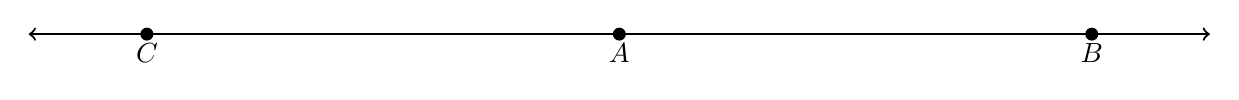
\begin{tikzpicture}[scale=1.5]
      \draw [->, thick] (0,0)--(-5,0);
      \draw [->, thick] (0,0)--(5,0);
      %\draw [->, thick] (0,0)--(-1.2,3);
      %\draw [fill] (-1,2.5) circle [radius=0.05] node[left ]{$B$};
      \draw [fill] (-4,0) circle [radius=0.05] node[below]{$C$};
      \draw [fill] (0,0) circle [radius=0.05] node[below]{$A$};
      \draw [fill] (4,0) circle [radius=0.05] node[below]{$B$};
    \end{tikzpicture}
    \end{center}
  \end{enumerate}


\subsubsection*{Angle pair short questions}
  \begin{enumerate}
    \item The sum of the measures of two supplementary angles equals $\rule{2cm}{0.15mm}$. \bigskip
    \item True or false: The angles making a linear pair are adjacent. $\rule{2cm}{0.15mm}$. \bigskip
    \item The sum of the measures of two complementary angles equals $\rule{2cm}{0.15mm}$. \bigskip
    \item True or false: The angles making a linear pair are complementary. $\rule{2cm}{0.15mm}$. \bigskip
    \item Two vertical angles are supplementary. What are their measures? $\rule{3cm}{0.15mm}$. \bigskip
    \item Sketch a linear pair.
    \end{enumerate}

  \begin{enumerate}
    \item \emph{variations}\\ True or false: The angles making a linear pair are supplementary. $\rule{2cm}{0.15mm}$. \bigskip
    \item The sum of the measures of two complementary angles equals $\rule{2cm}{0.15mm}$. \bigskip
    \item True or false: Vertical angles are congruent. $\rule{2cm}{0.15mm}$. \bigskip
    \item The sum of the measures of two supplementary angles equals $\rule{2cm}{0.15mm}$. \bigskip
    \item Two vertical angles are complementary. What are their measures? $\rule{3cm}{0.15mm}$. \bigskip
    \item Sketch a pair of vertical angles. \vspace{3cm}
    \end{enumerate}

\subsubsection*{Diagram short questions}
  \begin{enumerate}
    \item Given the situation in the diagram, answer each question. \vspace{1cm}
      \begin{flushright}
      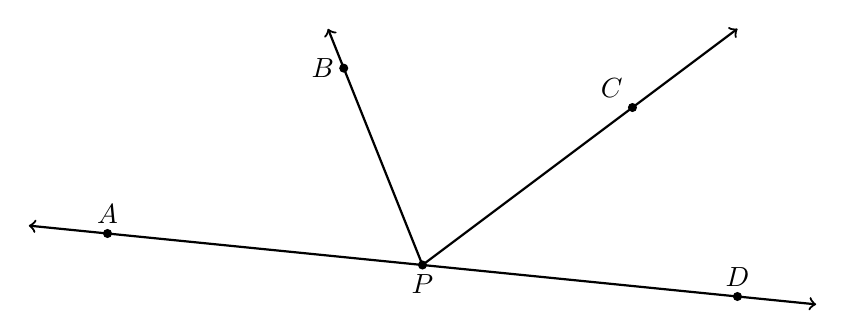
\begin{tikzpicture}[scale=1]
        \draw [->, thick] (0,0)--(4,3);
        \draw [<->, thick] (-5,.5)--(5,-.5);
        \draw [->, thick] (0,0)--(-1.2,3);
        \draw [fill] (-1,2.5) circle [radius=0.05] node[left ]{$B$};
        \draw [fill] (2.66666,2) circle [radius=0.05] node[above left ]{$C$};
        \draw [fill] (0,0) circle [radius=0.05] node[below]{$P$};
        \draw [fill] (4,-0.4) circle [radius=0.05] node[above]{$D$};
        \draw [fill] (-4,0.4) circle [radius=0.05] node[above]{$A$};
      \end{tikzpicture}
      \end{flushright}
    \begin{enumerate}
      \item True or false: $\overrightarrow{PA}$ and $\overrightarrow{PD}$ are opposite rays. $\rule{3cm}{0.15mm}$. \bigskip
      \item Name an angle adjacent to $\angle APB$. $\rule{3cm}{0.15mm}$. \bigskip
      \item True or false: $\angle APC$ and $\angle CPD$ are supplementary angles. $\rule{3cm}{0.15mm}$. \bigskip
      \item Name two angles that constitute a linear pair. $\rule{4cm}{0.15mm}$. \bigskip
    \end{enumerate}

    \item  \emph{(variation)} Given the situation in the diagram, answer each question. \vspace{1cm}
      \begin{flushright}
      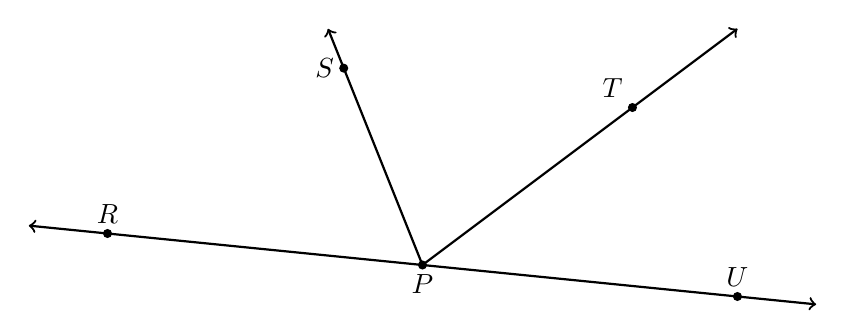
\begin{tikzpicture}[scale=1]
        \draw [->, thick] (0,0)--(4,3);
        \draw [<->, thick] (-5,.5)--(5,-.5);
        \draw [->, thick] (0,0)--(-1.2,3);
        \draw [fill] (-1,2.5) circle [radius=0.05] node[left ]{$S$};
        \draw [fill] (2.66666,2) circle [radius=0.05] node[above left ]{$T$};
        \draw [fill] (0,0) circle [radius=0.05] node[below]{$P$};
        \draw [fill] (4,-0.4) circle [radius=0.05] node[above]{$U$};
        \draw [fill] (-4,0.4) circle [radius=0.05] node[above]{$R$};
      \end{tikzpicture}
      \end{flushright}
    \begin{enumerate}
      \item True or false: $\overrightarrow{PR}$ and $\overrightarrow{PT}$ are opposite rays. $\rule{3cm}{0.15mm}$. \bigskip
      \item Name an angle adjacent to $\angle TPU$. $\rule{3cm}{0.15mm}$. \bigskip
      \item True or false: $\angle RPT$ and $\angle SPU$ are supplementary angles. $\rule{3cm}{0.15mm}$. \bigskip
      \item Name two angles that are adjacent. $\rule{4cm}{0.15mm}$. \bigskip
      \end{enumerate}
    \end{enumerate}

\subsubsection*{Complementary \& supplementary arithmetic}
  \begin{enumerate}
    \item Given two supplementary angles: $m \angle 1 = 50$, $m \angle 2 = x$.\\ Find $x$. %\vspace{2cm}
    \item Given two complementary angles: $m \angle 1 = x$, $m \angle 2 = 20$. Find $m \angle 1$. %\vspace{2cm}

    \item Given two supplementary angles: $m \angle 1 = 135$, $m \angle 2 = x$.\\ Find $x$. %\vspace{2cm}
    \item Given two complementary angles: $m \angle 1 = x$, $m \angle 2 = 75$. Find $m \angle 1$. %\vspace{2cm}

    \item Given $m \angle A=60$, $m \angle B=20$, $m \angle 1=30$, $m \angle DEF=150$, $m \angle FEG=10$. \bigskip
    \begin{enumerate}
      \item Find a pair of complementary angles. \rule{3cm}{0.15mm} \hspace{1cm} \rule{3cm}{0.15mm} \bigskip
      \item Find a pair of supplementary angles. \rule{3cm}{0.15mm} \hspace{1cm} \rule{3cm}{0.15mm} \bigskip
      \item Spicy: Find a different pair of supplementary angles. \rule{2cm}{0.15mm} \hspace{.5cm} \rule{2cm}{0.15mm}
      \end{enumerate}

    \end{enumerate}

\subsubsection*{Vertical angle algebra}
  \begin{enumerate}
    \item Given two vertical angles: $m \angle 1 = 3x+10$, $m \angle 2 = 2x+25$. Find $m \angle 1$.\\
    First label the drawing.
    \begin{flushright}
    \begin{tikzpicture}[scale=.7]
      \draw [<->, thick] (0,-1.5)--(10,1.5);
      \draw [<->, thick] (2,3.5)--(7,-3.5);
      \node at (3,.4){1};
      \node at (6,-.6){2};
      %\draw [fill] (0,0) circle [radius=0.05] node[below]{$P$};
      %\draw [fill] (6,0) circle [radius=0.05] node[below]{$R$};
      %\draw [fill] (3,0) circle [radius=0.05] node[below]{$Q$};
    \end{tikzpicture}
    \end{flushright}
    %\vspace{.5cm}
    \begin{enumerate}
      \item Write a geometric equation: \rule{4cm}{0.15mm} \hspace{1cm} \rule{4cm}{0.15mm}
      %\vspace{.7cm}
      \item Substitute algebraic values: \rule{4cm}{0.15mm}
      \item Solve for $x$
      %\vspace{2cm}
      %\begin{center} $x=$ \rule{1cm}{0.15mm} \end{center}
      \item Answer the question:
      %\vspace{2cm}
      \item Check your answer
      \end{enumerate}

  \item \emph{variation} Given two vertical angles: $m \angle 1 = 7x+10$, $m \angle 2 = 2x+45$. Find $m \angle 1$.\\
    First label the drawing.
    \begin{flushright}
    \begin{tikzpicture}[scale=.7]
      \draw [<->, thick] (0,-1.5)--(10,1.5);
      \draw [<->, thick] (2,3.5)--(7,-3.5);
      \node at (3,.4){1};
      \node at (6,-.6){2};
      %\draw [fill] (0,0) circle [radius=0.05] node[below]{$P$};
      %\draw [fill] (6,0) circle [radius=0.05] node[below]{$R$};
      %\draw [fill] (3,0) circle [radius=0.05] node[below]{$Q$};
    \end{tikzpicture}
    \end{flushright}

  \item \emph{variation} Given two perpendicular rays, $\overrightarrow{BA}$ and $\overrightarrow{BC}$, as shown. $m \angle ABD = 2x+10$, $m \angle DBC = x+5$. Find $m \angle DBC$.
    First label the drawing.
    \begin{flushright}
    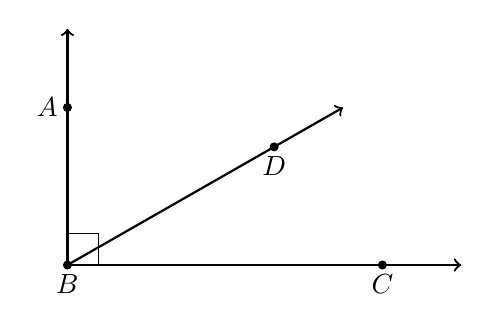
\begin{tikzpicture}[scale=1]
      \draw [<->, thick] (0,3)--(0,0)--(5,0);
      \draw [->, thick] (0,0)--(3.5, 2);
      \draw [-, thin] (0, 0.4)--(0.4, 0.4)--(0.4, 0);
      %\node at (3,.4){1};
      %\node at (6,-.6){2};
      \draw [fill] (0,0) circle [radius=0.05] node[below]{$B$};
      \draw [fill] (0,2) circle [radius=0.05] node[left]{$A$};
      \draw [fill] (4,0) circle [radius=0.05] node[below]{$C$};
      \draw [fill] (2.625, 1.5) circle [radius=0.05] node[below]{$D$};
    \end{tikzpicture}
    \end{flushright}

\subsubsection{Triangle external angles}

  \item Given $m\angle E=44$, and $m\angle GFH=112$. Find $m\angle G$.\\[1cm]
    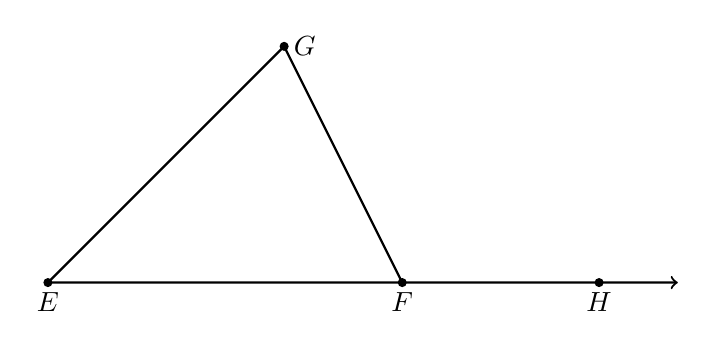
\begin{tikzpicture}
      %\draw [->, thick] (0,0)--(5,5);
      \draw [<-, thick] (8,0)--(0,0)--(3,3)--(4.5,0);
      \draw [fill] (0,0) circle [radius=0.05] node[below]{$E$};
      \draw [fill] (4.5,0) circle [radius=0.05] node[below]{$F$};
      \draw [fill] (3,3) circle [radius=0.05] node[right]{$G$};
      \draw [fill] (7,0) circle [radius=0.05] node[below]{$H$};
    \end{tikzpicture}
    %\vspace{4cm}

  \item Given  $\triangle EFG$ with $\overline{EF}$ extended to $A$. If $m\angle F=40^\circ$ and $m\angle AEG=140^\circ$, what is $m\angle EGF$?
    \begin{center}
      \begin{tikzpicture}%[scale=0.7]
        \draw [thick](0,0)node[below]{$A$}--
          (2,0)node[below]{$E$}--
          (8,0)node[below]{$F$}--
          (4,3)node[above]{$G$} --(2,0);
      \end{tikzpicture}
    \end{center}

  \item In  $\triangle ABC$ shown below, side $\overline{AC}$ is extended to point $D$ with $m\angle DAB=(180-2x)^\circ$, $m\angle C=(x-10)^\circ$, and $m\angle B=(3x+10)^\circ$.
    \begin{center}
      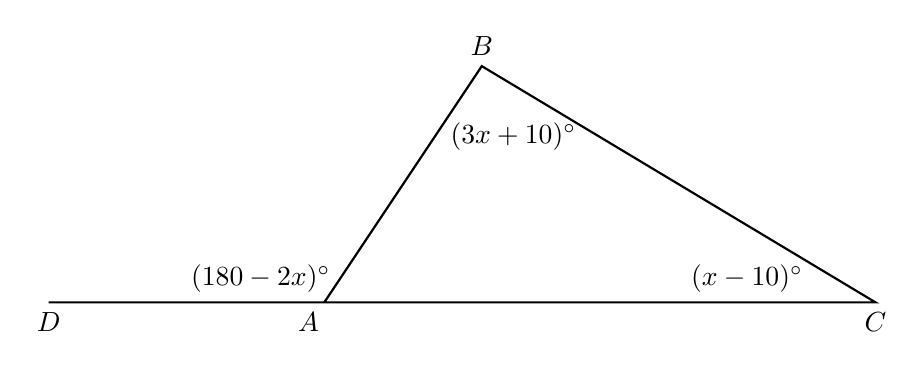
\begin{tikzpicture}
        \draw [thick](-1.5,0)node[below]{$D$}--
          (1.8,0)node[below]{$A$}--
          (9,0)node[below]{$C$}--
          (4,3)node[above]{$B$} --(2,0);
          \node at (2.2,0)[above left]{$(180-2x)^\circ$};
          \node at (8.2,0)[above left]{$(x-10)^\circ$};
          \node at (4.4,2.4)[below]{$(3x+10)^\circ$};
      \end{tikzpicture}
    \end{center}
    What is $m\angle BAC$?

  \item Spicy: Regents problem\\
    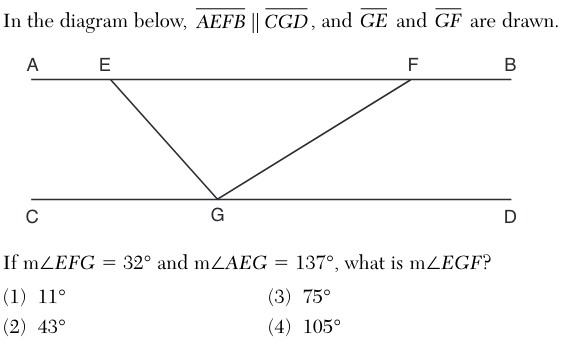
\includegraphics[width=0.75\textwidth]{4-3_ext-tri-sum.png}
    \vspace{2cm}

\end{enumerate}
\end{document}
